%%%%%%%%%%%%%%%%%%%%%%%%%%%%%%%%%%%%%%%%%%%%%%%%%%%%%%%%%%%%%%%%%%%%%%%%%%%%%%%%%%%%
% Document data
%%%%%%%%%%%%%%%%%%%%%%%%%%%%%%%%%%%%%%%%%%%%%%%%%%%%%%%%%%%%%%%%%%%%%%%%%%%%%%%%%%%%
\documentclass[12pt]{article} %report allows for chapters
%%%%%%%%%%%%%%%%%%%%%%%%%%%%%%%%%%%%%%%%%%%%%%%%%%%%%%%%%%%%%%%%%%%%%%%%%%%%%%%%%%%%
\usepackage{preamble}
\newcommand{\vecx}{\boldsymbol{\vec{x}}}
\newcommand{\vecy}{\boldsymbol{\vec{y}}}

\begin{document}

\begin{center}
   \textsc{\large MATH 271, Worksheet 9, \emph{Solutions.}}\\
   \textsc{Linear independence, span, and bases. Matrix determinants and traces.}
\end{center}
\vspace{.5cm}



\begin{problem}
Consider the following three vectors $\vecu,\vecv,\vecw\in \R^3$ given by
\[
\vecu = \xhat + \yhat +\zhat, \qquad \vecv = 2\xhat + \yhat + 2\zhat, \qquad \vecw = -2\xhat + \yhat +\zhat. 
\]
\begin{enumerate}[(a)]
    \item We can write a linear combination of these vectors by taking
    \[
    \alpha \vecu + \beta \vecv + \gamma \vecw,
    \]
    where $\alpha,\beta,\gamma \in \R$.  Write this linear combination as a matrix times a vector.
    \item Are these vectors linearly independent?
    \item Does this list of vectors form a basis for $\R^3$? \emph{Hint: use the above work. Can any vector in $\R^3$ be written as a linear combination of these vectors?}
\end{enumerate}
\end{problem}
\begin{solution}
    \begin{enumerate}[(a)]
        \item We note that a matrix $[A]$ times a vector $\vecx$ takes linear combinations of the columns. So if we take
        \[
            [A] = \begin{pmatrix} \vert & \vert & \vert \\ \vecu & \vecv & \vecw \\ \vert & \vert & \vert \end{pmatrix} \qquad \textrm{and} \qquad \vecx = \begin{pmatrix} \alpha \\ \beta \\ \gamma \end{pmatrix},
        \]
        then we have
        \[
        [A]\vecx = \alpha \vecu + \beta \vecv + \gamma \vecw,
        \]
        as intended. This is convenient as it allows us to determine properties about sets of vectors using computational techniques like row reduction or the determinant.
        \item To see that these vectors are linearly independent we must show that
        \[
        \alpha \vecu + \beta \vecv + \gamma \vecw = \zerovec,
        \]
        is true if and only if $\alpha,\beta,\gamma = 0$ is the only possible solution.  In other words, the only solution to the homogeneous equation
        \[
        [A]\vecx = \zerovec,
        \]
        is trivial (i.e., $\operatorname{Null}([A])$ contains only the zero vector).  To see this, we form the augmented matrix then row reduce. We have
        \[
        \left( \begin{tabular}{ccc|c} 1 & 2 & -2 & 0 \\ 1 & 1 & 1 & 0 \\ 1 & 2 & 1 & 0 \end{tabular} \right),
        \]
        which reduces down to
        \[
        \left( \begin{tabular}{ccc|c} 1 & 0 & 0 & 0\\ 0 & 1 & 0 & 0\\ 0 & 0 & 1 & 0\end{tabular} \right),
        \]
        to yield the equations $\alpha = 0$, $\beta = 0$, and $\gamma=0$.  Thus, $\vecu$, $\vecv$, and $\vecw$ constitute a linearly independent set of vectors.

        \item We have already shown the necessary work above.  Since the matrix $[A]$ can be row reduced to the $3\times 3$ identity matrix $[I]$, we know this is possible.  Take an arbitrary vector $\vecy = y_1 \xhat + y_2\yhat + y_3\zhat$ and consider the inhomogeneous equation
        \[
        [A]\vecx = \vecy.
        \]
        If we are able to find a solution given this arbitrary $\vecy$, then $\vecu$, $\vecv$, and $\vecw$ span $\R^3$.  We take again the augmented matrix
        \[
        \left( \begin{tabular}{ccc|c} 1 & 2 & -2 & $y_1$ \\ 1 & 1 & 1 & $y_2$ \\ 1 & 2 & 1 & $y_3$ \end{tabular} \right)
        \]
        and row reduce to
        \[
\left( \begin{tabular}{ccc|c} 1 & 0 & 0 & $\frac{y_1}{3} + 2y_2 - \frac{4y_3}{3}$ \\ 0 & 1 & 0 & $y_3 - y_2$\\ 0 & 0 & 1 & $\frac{y_3 -y_1}{3}$ \end{tabular} \right).
        \]
        Thus we have found solutions for $\alpha$, $\beta$, and $\gamma$ and it must be that $\vecu$, $\vecv$, and $\vecw$ span $\R^3$ and moreover provide a basis for $\R^3$ since they are also linearly independent.  
    \end{enumerate}
\begin{remark}
    One can see that all of this really amounts to just row reducing the matrix $[A]$.  If we can reduce this matrix to the identity matrix (as in this problem), that tells us all that we need to know.  We will do this for the next problem but you should have the intuition on why that suffices from this problem.
\end{remark}
\end{solution}

\newpage
\begin{problem}
Consider the following three vectors $\vecu,\vecv,\vecw\in \R^3$ given by
\[
\vecu = \xhat + \yhat +\zhat, \qquad \vecv = \xhat + \yhat, \qquad \vecw = 2\xhat + 2\yhat +\zhat. 
\]
\begin{enumerate}[(a)]
    \item We can write a linear combination of these vectors by taking
    \[
    \alpha \vecu + \beta \vecv + \gamma \vecw,
    \]
    where $\alpha,\beta,\gamma \in \R$.  Write this linear combination as a matrix times a vector.
    \item Are these vectors linearly independent?
    \item Does this list of vectors form a basis for $\R^3$? \emph{Hint: use the above work. Can any vector in $\R^3$ be written as a linear combination of these vectors?}
\end{enumerate}
\end{problem}
\begin{solution}
Given our work in the previous problem, we can cut down significantly on the work for this problem seeing as it is analogous.
    \begin{enumerate}[(a)]
        \item We take
        \[
            [A] = \begin{pmatrix} 1 & 1 & 2 \\ 1 & 1 & 2 \\ 1 & 0 & 1 \end{pmatrix} \qquad \textrm{and} \qquad \vecx = \begin{pmatrix} \alpha \\ \beta \\ \gamma \end{pmatrix},
        \]
        and note $[A]\vecx$ gives us the intended linear combination.
        
        \item We simply row reduce $[A]$ to get 
        \[
        \begin{pmatrix} 1 & 0 & 1 \\ 0 & 1 & 1 \\ 0 & 0 & 0 \end{pmatrix}.
        \]
        So these vectors are not linearly independent since we have a row of zeros.
        \item No, the vectors are not a basis for $\R^3$ as they are not linearly independent. In fact, they do not span $\R^3$ either.
    \end{enumerate}
\end{solution}

\newpage
\begin{problem}
Compute the determinants of the matrices you found in Problems 1 and 2.  Explain how this gives insight on your ability to find solutions to inhomogeneous and homogeneous equations with those matrices.
\end{problem}
\begin{solution}
Let $[A]_1$ and $[A]_2$ be the matrices from Problem 1 and 2 respectively.  Expanding across row 1 for $[A]_1$ we find
\begin{align*}
\det ([A]_1) &= 1 \left| \begin{tabular}{cc} 1 & 1 \\ 2 & 1 \end{tabular} \right| - 2 \left| \begin{tabular}{cc} 1 & 1 \\ 1 & 1 \end{tabular} \right| - 2 \left| \begin{tabular}{cc} 1 & 1 \\ 1 & 2 \end{tabular} \right|\\
&=-1+0-2 = -3.
\end{align*}
Likewise for $[A]_2$ we have
\begin{align*}
\det ([A]_2) &= 1 \left| \begin{tabular}{cc} 1 & 2 \\ 0 & 1 \end{tabular} \right| - 1 \left| \begin{tabular}{cc} 1 & 2 \\ 1 & 1 \end{tabular} \right| + 2 \left| \begin{tabular}{cc} 1 & 1 \\ 1 & 0 \end{tabular} \right|\\
&=1+1-2 = 0.
\end{align*}

Since the determinant for $[A]_1$ is nonzero, we know that we will only have the trivial solution to the homogeneous equation.  This is due to the fact that the columns must be linearly independent if the determinant is nonzero and we showed this more explicitly in Problem 1.  In the same vein, we can find unique solutions to any inhomogeneous equation since we have three linearly independent columns.  Thinking of the columns as vectors in $\R^3$, we can note that three linearly independent vectors constitute a basis for $\R^3$.

The determinant of $[A]_2$ is zero, so the columns are dependent. In fact, one can see that $\vecu+\vecv = \vecw$ if we look back towards Problem 2 where we also found that there is a nontrivial solution for the homogeneous equation due to the form of the row reduced matrix (there is a whole row of zeros and therefore we have a free variable).  Since we only have two linearly independent vectors in $\R^3$, we cannot possibly span all of $\R^3$ and so there is some inhomogeneous equation we can't solve.  For example, take $\vecy=3\xhat +2\yhat+\zhat$ and note that $\vecy = \vecw + \xhat$.  Check for yourself that there is no corresponding solution $\vecx$ for this given $\vecy$.
\end{solution}

\newpage
\begin{problem}
Suppose we have a matrix $[A]$ such that $[A]\vecu = \lambda \vecu$ for some constant $\lambda$.  Suppose as well that $\vecv$ satisfies the same equation in that $[A]\vecv = \lambda \vecv$.  Finally, suppose there exists a vector $\vecw$ that satisfies a similar equation $[A]\vecw = \eta \vecw$ but with $\eta\neq \lambda$.
\begin{enumerate}[(a)]
    \item Show that any vector in the span of $\vecu$ and $\vecv$ also satisfies the same equation as $\vecu$ and $\vecv$.
    \item Show that the span of $\vecu$ and $\vecw$ does not solve either of the given equations.
\end{enumerate}
\end{problem}
\begin{solution}~
    \begin{enumerate}[(a)]
        \item An arbitrary vector $\vecx$ in the span of $\vecu$ and $\vecv$ can be written as
        \[
        \vecx = \alpha \vecu + \beta \vecv,
        \]
        for arbitrary scalars $\alpha,\beta \in \R$.  We show now that $\vecx$ satisfies the same equation that $\vecu$ and $\vecv$ do, namely that $[A]\vecx = \lambda \vecx$.  We have
        \begin{align*}
                [A]\vecx = [A](\alpha \vecu + \beta \vecv) &= \alpha [A]\vecu + \beta [A]\vecv\\
                &= \alpha \lambda \vecu + \beta \lambda \vecv\\
                &= \lambda \vecx.
        \end{align*}
        
        \item Consider now an arbitrary vector in the span of $\vecu$ and $\vecw$ given by $\vecx = \alpha \vecu + \beta \vecw$ for arbitrary $\alpha,\beta \in \R$.  We have
        \begin{align*}
            [A]\vecx = [A](\alpha\vecu + \beta \vecw) &= \alpha [A]\vecu + \beta [A]\vecw\\
            &= \alpha \lambda \vecu + \beta \eta \vecw.
        \end{align*}
        Now, since $\lambda \neq \eta$, we cannot factor out these constants like we did in part (a), and so $\vecx$ here does not satisfy either of the given equations.  In fact, the same would be true for any vector in the span of $\vecv$ and $\vecw$ as well.  
    \end{enumerate}
\begin{remark}
    This concept is actually fairly important.  The equations that $\vecu$, $\vecv$, and $\vecw$ satisfy are eigenvalue equations (which we will cover soon).  It shows that for different eigenvalues ($\lambda \neq \eta$) that the corresponding eigenvectors ($\vecu$ and $\vecv$ for $\lambda$ and $\vecw$ for $\eta$) do not add together to yield another eigenvector. This is only true when the eigenvalues are the same, as in the case for part (a) where we saw vectors in the span of $\vecu$ and $\vecv$ did satisfy the same eigenvalue equation.
\end{remark}
\end{solution}

\newpage
\begin{problem}
Consider the matrix 
\[
[J] = \begin{pmatrix} 0 & -1 \\ 1 & 0 \end{pmatrix},
\]
which acts as a counter clockwise rotation by $\pi/2$ in the $xy$-plane.  
\begin{enumerate}[(a)]
    \item Show that $\det([J])=1$.
    \item Explain why $[J]$ does not distort areas using what you know about the determinant.
    \item Consider a new matrix $[J]-\lambda [I]$ where $[I]$ is the $2\times 2$ identity matrix and $\lambda$ is a scalar variable.  Compute $\det([J]-\lambda [I])$. This is called the \emph{characteristic polynomial}.
    \item Find the roots of the characteristic polynomial.
\end{enumerate}
\end{problem}
\begin{solution} This matrix is fundamentally important.  In a homework problem, we saw that this matrix gives rise to ways of representing the algebra of complex numbers $\C$ using real $2\times 2$ matrices.  It is also a building block for creating higher dimensional rotation matrices which we see here in Problem 10.
\begin{enumerate}[(a)]
    \item We have  
    \[
        \det([J])=0+1 = 1.
    \]
    \item First, if the matrix $[J]$ acts solely by rotation, we do not expect areas to change under the action of $[J]$. Note that $[J]$ is merely a representation of the linear transformation $J$.  We construct $[J]$ as
    \[
        [J] = \begin{pmatrix} \vert & \vert \\ J(\xhat) & J(\yhat) \\ \vert & \vert \end{pmatrix}.
    \]
    Thus, the columns of $[J]$ are transformations of the basis vectors $\xhat$ and $\yhat$.  If we have
    \[
        [I] = \begin{pmatrix} \vert & \vert \\ \xhat & \yhat \\ \vert & \vert \end{pmatrix} = \begin{pmatrix} 1 & 0 \\ 0 & 1 \end{pmatrix},
    \]
    we can note that $\det([I])=1$, so the area of the parallelogram created from $\xhat$ and $\yhat$ is 1.  Drawing this in the plane, this can be quickly realized.
            \[
        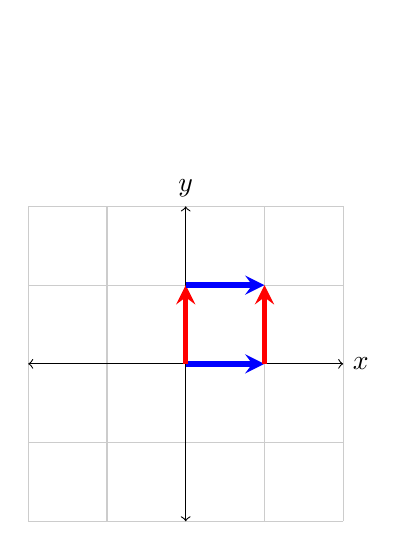
\begin{tikzpicture}
        \draw[thin,gray!40] (-2,-2) grid (2,2);
        \draw[<->] (-2,0)--(2,0) node[right]{$x$};
        \draw[<->] (0,-2)--(0,2) node[above]{$y$};
        \draw[line width=2pt,blue,-stealth](0,0)--(1,0) node[anchor=north] at (.5,0){$\xhat$};
        \draw[line width=2pt, red, -stealth](0,0)--(0,1) node[anchor=east] at (0,.5){$\yhat$};
        \draw[line width=2pt, blue, -stealth](0,1)--(1,1) node[anchor=north] at (1,4){};
        \draw[line width=2pt, red, -stealth](1,0)--(1,1) node[anchor=south] at (1,4){};
        \end{tikzpicture}
        \]
    The transformed vectors $J(\xhat)=\yhat$ and $J(\yhat)=-\xhat$ then create the parallelogram in the plane below.
            \[
        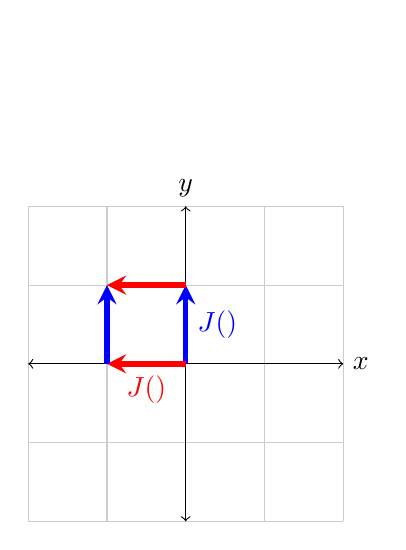
\begin{tikzpicture}
        \draw[thin,gray!40] (-2,-2) grid (2,2);
        \draw[<->] (-2,0)--(2,0) node[right]{$x$};
        \draw[<->] (0,-2)--(0,2) node[above]{$y$};
        \draw[line width=2pt,blue,-stealth](0,0)--(0,1) node[anchor=west] at (0,.5){$J(\xhat)$};
        \draw[line width=2pt, red, -stealth](0,0)--(-1,0) node[anchor=north] at (-.5,0){$J(\yhat)$};
        \draw[line width=2pt, red, -stealth](0,1)--(-1,1) node[anchor=north] at (1,4){};
        \draw[line width=2pt, blue, -stealth](-1,0)--(-1,1) node[anchor=south] at (1,4){};
        \end{tikzpicture}
        \]
    We realize now that the parallelogram we had prior was only rotated and the area of the transformed parallelogram is unchanged. So, $[J]$ does not distort areas.

    \item We have
    \[
        [J] - \lambda [I] = \begin{pmatrix} -\lambda & -1 \\ 1 & -\lambda \end{pmatrix}.
    \]
    Then,
    \[
        \det([J]-\lambda[I]) = \lambda^2 + 1.
    \]
    \item The roots to the polynomial from (c) are then solutions to 
    \[
    \lambda^2+1=0.
    \]
    The solutions are $\pm i$ which goes back to the idea that $[J]$ represents the complex number $i$ in some way.
\end{enumerate}
\end{solution}

\newpage
\begin{problem}
Consider the matrices
\[
[A] = \begin{pmatrix} 0 & 3 \\ 2 & 0 \end{pmatrix}, \quad [B] = \begin{pmatrix} 3 & -1 \\ 1 & 2 \end{pmatrix}, \quad [C] = \begin{pmatrix} 3 & 2 \\ 3 & 2 \end{pmatrix}.
\]
\begin{enumerate}[(a)]
    \item Compute the determinant of each matrix.
    \item For each matrix, draw the vectors $\xhat$ and $\yhat$ and draw the transformed vectors (the matrix applied to $\xhat$ and $\yhat$). Explain how the matrices transform areas and relate this back to the determinant of the matrices.  Do this in a different plane for each matrix to avoid making this look messy.
\end{enumerate}
\end{problem}
\begin{solution} This problem is intended to show that the determinant (up to a $\pm$ sign) provides us the ``stretch" factor that a matrix causes.  To be precise, the sign comes from a change in orientation and the absolute value of the determinant tells us how volume is transformed.  That is, how areas (or volumes in higher dimensions) are stretched and squished by a matrix. We will realize that determinants of zero correspond to completely squishing at least one direction down to zero completely.
    \begin{enumerate}[(a)]
        \item The determinants are
        \begin{align*}
        \det([A]) &= -6,\\
        \det([B]) &= 5,\\
        \det([B]) &= 0.
        \end{align*}
        \item We first begin by drawing the vectors $\xhat$ and $\yhat$ and the parallelogram that they generate and then for the the first matrix $[A]$, we have $[A]\xhat = 3\yhat$ and $[A]\yhat = 2\xhat$, and we can draw these transformed vectors.
        \[
        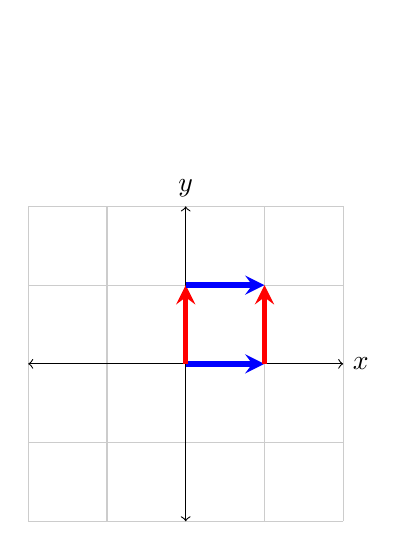
\begin{tikzpicture}
        \draw[thin,gray!40] (-2,-2) grid (2,2);
        \draw[<->] (-2,0)--(2,0) node[right]{$x$};
        \draw[<->] (0,-2)--(0,2) node[above]{$y$};
        \draw[line width=2pt,blue,-stealth](0,0)--(1,0) node[anchor=north] at (.5,0){$\xhat$};
        \draw[line width=2pt, red, -stealth](0,0)--(0,1) node[anchor=east] at (0,.5){$\yhat$};
        \draw[line width=2pt, blue, -stealth](0,1)--(1,1) node[anchor=north] at (1,4){};
        \draw[line width=2pt, red, -stealth](1,0)--(1,1) node[anchor=south] at (1,4){};
        \end{tikzpicture}
        \quad \xrightarrow{\textrm{apply }[A]} \quad
        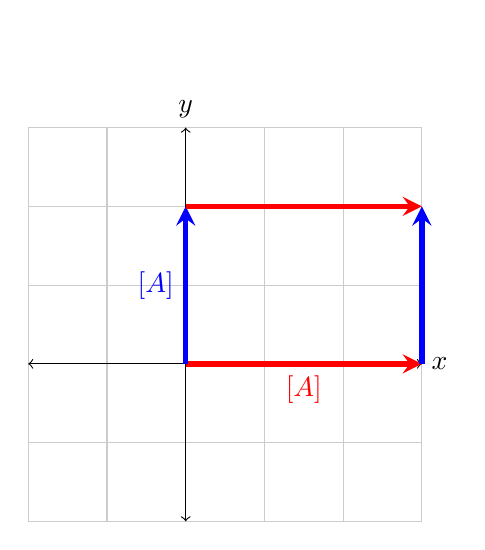
\begin{tikzpicture}
        \draw[thin,gray!40] (-2,-2) grid (3,3);
        \draw[<->] (-2,0)--(3,0) node[right]{$x$};
        \draw[<->] (0,-2)--(0,3) node[above]{$y$};
        \draw[line width=2pt,red,-stealth](0,0)--(3,0) node[anchor=north] at (1.5,0){$[A]\yhat$};
        \draw[line width=2pt, blue, -stealth](0,0)--(0,2) node[anchor=east] at (0,1){$[A]\xhat$};
        \draw[line width=2pt, red, -stealth](0,2)--(3,2) node[anchor=north] at (1,4){};
        \draw[line width=2pt, blue, -stealth](3,0)--(3,2) node[anchor=south] at (1,4){};
        \end{tikzpicture}
        \]
        We see clearly now that the area of the transformed parallelogram has grown by a factor of $6=|\det([A])$ and the orientation was reversed in this case. To see what I mean by orientation, briefly picture these vectors in $\R^3$ and we note $\xhat \times \yhat = \zhat$ whereas $[A]\xhat \times [A]\yhat = -6\zhat$.  This orientation can be realized as well by using the right hand rule.
        
        \item We now do the same for $[B]$ and we have $[B]\xhat = 3\xhat + \yhat$ and $[B]\yhat = -\xhat + 2\yhat$.
        \[
        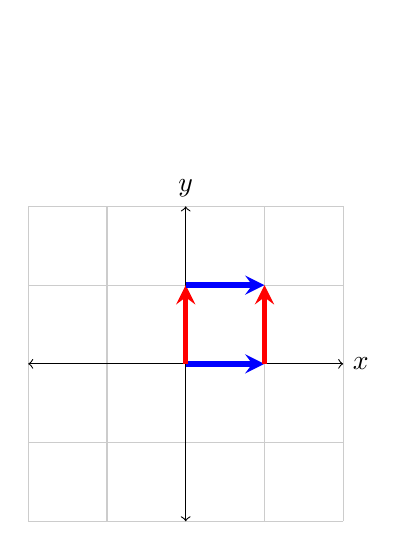
\begin{tikzpicture}
        \draw[thin,gray!40] (-2,-2) grid (2,2);
        \draw[<->] (-2,0)--(2,0) node[right]{$x$};
        \draw[<->] (0,-2)--(0,2) node[above]{$y$};
        \draw[line width=2pt,blue,-stealth](0,0)--(1,0) node[anchor=north] at (.5,0){$\xhat$};
        \draw[line width=2pt, red, -stealth](0,0)--(0,1) node[anchor=east] at (0,.5){$\yhat$};
        \draw[line width=2pt, blue, -stealth](0,1)--(1,1) node[anchor=north] at (1,4){};
        \draw[line width=2pt, red, -stealth](1,0)--(1,1) node[anchor=south] at (1,4){};
        \end{tikzpicture}
        \quad \xrightarrow{\textrm{apply }[B]} \quad
        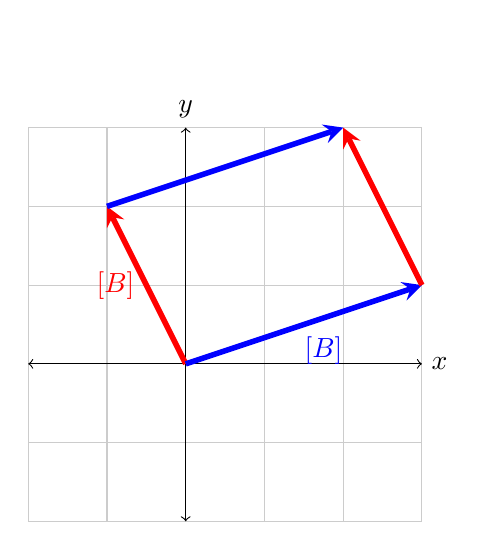
\begin{tikzpicture}
        \draw[thin,gray!40] (-2,-2) grid (3,3);
        \draw[<->] (-2,0)--(3,0) node[right]{$x$};
        \draw[<->] (0,-2)--(0,3) node[above]{$y$};
        \draw[line width=2pt,red,-stealth](0,0)--(-1,2) node[anchor=east] at (-.5,1){$[B]\yhat$};
        \draw[line width=2pt, blue, -stealth](0,0)--(3,1) node[anchor=north] at (1.75,.5){$[B]\xhat$};
        \draw[line width=2pt, red, -stealth](3,1)--(2,3) node[anchor=north] at (1,4){};
        \draw[line width=2pt, blue, -stealth](-1,2)--(2,3) node[anchor=south] at (1,4){};
        \end{tikzpicture}
        \]
        The orientation is not changed here and the area of the new parallelogram is 5.

        \item Now, the determinant of $[C]$ is zero, so we expect to find zero area when we apply the transformation. First, we have $[C]\xhat = 3\xhat + 3\yhat$ and $[C]\yhat = 2\xhat + 2\yhat$.  This gives us the following picture.
        \[
        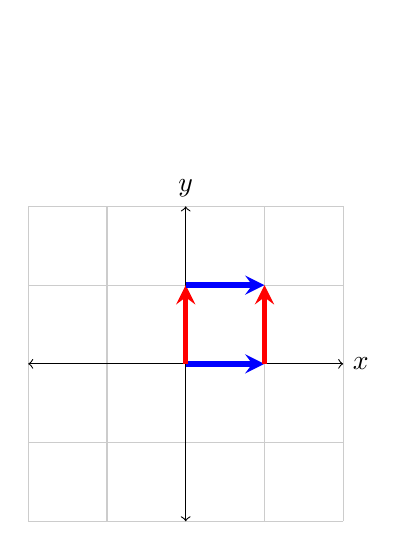
\begin{tikzpicture}
        \draw[thin,gray!40] (-2,-2) grid (2,2);
        \draw[<->] (-2,0)--(2,0) node[right]{$x$};
        \draw[<->] (0,-2)--(0,2) node[above]{$y$};
        \draw[line width=2pt,blue,-stealth](0,0)--(1,0) node[anchor=north] at (.5,0){$\xhat$};
        \draw[line width=2pt, red, -stealth](0,0)--(0,1) node[anchor=east] at (0,.5){$\yhat$};
        \draw[line width=2pt, blue, -stealth](0,1)--(1,1) node[anchor=north] at (1,4){};
        \draw[line width=2pt, red, -stealth](1,0)--(1,1) node[anchor=south] at (1,4){};
        \end{tikzpicture}
        \quad \xrightarrow{\textrm{apply }[B]} \quad
        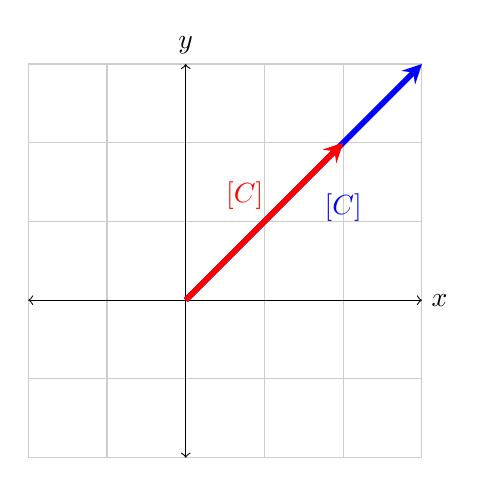
\begin{tikzpicture}
        \draw[thin,gray!40] (-2,-2) grid (3,3);
        \draw[<->] (-2,0)--(3,0) node[right]{$x$};
        \draw[<->] (0,-2)--(0,3) node[above]{$y$};
        \draw[line width=2pt, blue, -stealth](0,0)--(3,3) node[anchor=north] at (2,1.5){$[C]\xhat$};
        \draw[line width=2pt,red,-stealth](0,0)--(2,2) node[anchor=south] at (.75,1){$[C]\yhat$};
        \end{tikzpicture}
        \]
        So we see now that $[C]\xhat$ lies on the same line as $[C]\yhat$ and so there cannot be a parallelogram made from this. So the area has been squished down to zero.
    \end{enumerate}
\end{solution}

\newpage
\begin{problem}
Consider the vectors in $\R^3$, $\vecu=3\xhat - \yhat + 4\zhat$ and $\vecv=-\yhat - 2\zhat$.  Show that $\tr(\vecu \vecv^\top) = \vecu^\top \vecv$.
\end{problem}
\begin{solution}
We first compute the matrix products
\[
\vecu \vecv^\top = \begin{pmatrix} 3 \\ -1 \\ 4 \end{pmatrix} \begin{pmatrix} 0 & -1 & -2 \end{pmatrix} = \begin{pmatrix} 0 & -3 & -6 \\ 0 & 1 & 2 \\ 0 & -4 & -8 \end{pmatrix}
\]
and
\[
\vecu^\top \vecv= \begin{pmatrix} 3 & -1 & 4 \end{pmatrix} \begin{pmatrix} 0 \\ -1 \\ -2 \end{pmatrix} = -7.
\]
Now, take the trace of the first product
\[
\tr(\vecu \vecv^\top) = -7.
\]
\end{solution}

\newpage
\begin{problem}
Prove the previous problem for two arbitrary vectors in $\R^n$.
\end{problem}
\begin{solution}
    Let $\vecu = u_1 \xhat_1 + u_2 \xhat_2 + \cdots u_n \xhat_n$ and $\vecv = v_1 \xhat_1 + v_2 \xhat_2 + \cdots + v_n \xhat_n$. Now, consider two matrices $[A]$ and $[B]$ with entries $a_{ij}$ and $b_{ij}$ respectively. If we multiply $[A]$ and $[B]$, the output matrix $[C] = [A][B]$ has coefficients $c_{ij}$ given by the expression
    \[
        c_{ij} = \sum_{k=1}^n a_{ik}b_{kj}.
    \]
    In our case, we let $[A]=\vecu$ be a $n\times 1$ matrix and $[B]=\vecv$ be a $1\times n$ matrix, so we no longer need the sum as $k=1$ is the only option in this case. Thus,
    \[
        c_{ij} = \vecu_i \vecv_j = u_i u_j,
    \]
    and the diagonal elements are then $c_{ii} = u_i v_i$ and the trace is then
    \[
        \tr([C]) = \sum_{i=1}^n u_i v_i = \vecu \cdot \vecv.
    \]
    We note that $\vecu \cdot \vecv = \vecu^\top \vecv$ and we have proven the result.
\end{solution}

\newpage
\begin{problem}
Is it true that $\tr([A]^\top)=\tr([A])$ for any matrix? Why or why not?
\end{problem}
\begin{solution}
    Yes, this is true.  Given a matrix $[A]$ with entries $a_{ij}$ we have that the components of $[A]^\top$ are $a_{ji}$ (we have swapped rows and columns).  But, we note that this leaves the diagonal entries $a_{ii}$ unaffected and since the trace is the sum of the diagonal elements ($\tr([A]) = \sum_{i=1}^n a_{ii}$), the trace is not changed either.
\end{solution}

\newpage
\begin{problem}
Consider the linear transformations on $\R^3$ to $\R^3$ given by
\begin{align*}
    R_x(\theta) &= \begin{pmatrix} 1 & 0 & 0 \\ 0 & \cos\theta & -\sin \theta \\ 0 & \sin\theta & \cos \theta \end{pmatrix}\\
    R_y(\theta) &= \begin{pmatrix} \cos \theta & 0 & \sin \theta \\ 0 & 1 & 0 \\ -\sin \theta & 0 & \cos \theta \end{pmatrix}\\
    R_z(\theta) &= \begin{pmatrix} \cos \theta & -\sin \theta & 0 \\ \sin \theta & \cos \theta  & 0 \\ 0 & 0 & 1 \end{pmatrix}.
\end{align*}
\textbf{Fact:} These matrices are generators for the \emph{group of rotations} $\SO(3)$ of $\R^3$.
\begin{enumerate}[(a)]
    \item Let $\theta = \pi/2$. Show that $R_x(\pi/2)$ rotates a vector counter clockwise by $\pi/2$ radians around the $x$-axis.
    \item Show that the determinant of each of these matrices is 1 for any value of $\theta$.
    \item Using properties of determinants, show that the determinant of a product of rotation matrices is also 1.
    \item Explain geometrically why a rotation matrix must have a determinant of 1.
    \item Show that $R_x(\theta)R_x(\theta)^\top = I$. This in fact true for any rotation matrix.
\end{enumerate}
\end{problem}
\begin{solution} Rotations are important symmetries of space.  Physical laws tend to be invariant under the symmetries of space, and these matrices show up as a means of representing the symmetries that we expect physical laws to have.
    \begin{enumerate}[(a)]
        \item  Previously, we have found that a counter clockwise rotation by $\pi/2$ in the $xy$-plane is given by letting $\xhat \to \yhat$ and $\yhat \to -\xhat$ as we have seen with the matrix $[J]$.  Now, a rotation of $\pi/2$ about the $x$-axis corresponds to a rotation by $\pi/2$ in the $yz$-plane.  In particular we should have $\xhat \to \xhat$ stays put and $\yhat \to \zhat$ and $\zhat \to -\yhat$.  Now we have
        \[ 
            R_x(\pi/2) = \begin{pmatrix} 1 & 0 & 0 \\ 0 & 0 & -1 \\ 0 & 1 & 0 \end{pmatrix}.
        \]
        Then, we get $R_x(\pi/2)\xhat = \xhat$, $R_x(\pi/2)\yhat = \zhat$ and $R_x(\pi/2)\zhat = -\yhat$ as intended.
        \item We have
        \[
        \det(R_x(\theta)) = 1 \left| \begin{tabular}{cc} $\cos \theta$ & $-\sin \theta$ \\ $\sin \theta$ & $\cos \theta$ \end{tabular} \right| = \cos^2 \theta + \sin^2 \theta = 1,
        \]
        by expanding across the top row. Similarly,
                \[
        \det(R_y(\theta)) = 1 \left| \begin{tabular}{cc} $\cos \theta$ & $\sin \theta$ \\ $-\sin \theta$ & $\cos \theta$ \end{tabular} \right|  = 1,
        \]
        by expanding across the middle row and finally
        \[
        \det(R_z(\theta)) = 1 \left| \begin{tabular}{cc} $\cos \theta$ & $-\sin \theta$ \\ $\sin \theta$ & $\cos \theta$ \end{tabular} \right|  = 1,
        \]
        by expanding across the bottom row.
        \item Determinants are multiplicative so we get
        \[
            \det(R_x(\theta)R_y(\phi) R_z(\omega)) = \det(R_x(\theta)) \det(R_y(\phi)) \det(R_z(\omega)) = 1.
        \]
        \item A rotation does not stretch or squish any directions, it only rotates them.  So the determinant must be $\pm 1$.  Since a rotation does not change orientation (right-handedness) of the basis vectors, it is indeed $+1$.
        \item We have
        \begin{align*}
R_x(\theta)R_x(\theta)^\top &= \begin{pmatrix} 1 & 0 & 0 \\ 0 & \cos\theta & -\sin \theta \\ 0 & \sin\theta & \cos \theta \end{pmatrix} \begin{pmatrix} 1 & 0 & 0 \\ 0 & \cos\theta & \sin \theta \\ 0 & -\sin\theta & \cos \theta \end{pmatrix} \\&= \begin{pmatrix} 1 & 0 & 0 \\ 0 & \cos^2 \theta + \sin^2 \theta & \cos\theta \sin \theta - \cos \theta \sin \theta\\ 0 & \cos\theta \sin \theta - \cos \theta \sin \theta & \cos^2 \theta + \sin^2 \theta \end{pmatrix}\\ &= [I].
        \end{align*}
    \end{enumerate}
\end{solution}

\newpage
\begin{problem}
Consider the matrix 
\[
M = \begin{pmatrix} 1 & 2 & 3 \\ 4 & 5 & 6 \\ 7 & 8 & 9 \end{pmatrix}.
\]
\begin{enumerate}[(a)]
    \item Compute $\tr(M)$. 
    \item Compute $M^{R_x}=R_x(\pi/2)MR_x(\pi/2)^\top$.
    \item What is the trace of $M^{R_x}$?
    \item Can you see why you have the answer in (c) from properties of the trace?
\end{enumerate}
\end{problem}
\begin{solution}~
\begin{enumerate}[(a)]
    \item We have
    \[
    \tr(M) = 1 + 5 + 9 = 15.
    \]
    \item We take
    \begin{align*}
    M^{R_x} &= \begin{pmatrix} 1 & 0 & 0 \\ 0 & 0 & -1 \\ 0 & 1 & 0 \end{pmatrix} \begin{pmatrix} 1 & 2 & 3 \\ 4 & 5 & 6 \\ 7 & 8 & 9 \end{pmatrix} \begin{pmatrix} 1 & 0 & 0 \\ 0 & 0 & 1 \\ 0 & -1 & 0 \end{pmatrix}\\
    &=\begin{pmatrix} 1 & -3 & 2 \\ -7 & 9 & -8 \\ 4 & -6 & 5 \end{pmatrix}.
    \end{align*}
    \item We get
    \[
    \tr\left( M^{R_x}\right) = 15,
    \]
    which is the same as $\tr(M)$.
    \item We have
    \begin{align*}
        \tr\left(M^{R_x}\right) &= \tr(R_x(\pi/2) M R_x(\pi/2)^\top) \\
        &= \tr(M R_x(\pi/2)^\top R_x(\pi/2)),
    \end{align*}
    by the properties of the trace.  Then note $R_x(\pi/2)^\top R_x(\pi/2)=[I]$ by work analogous to the previous problem and so
    \[
    \tr\left(M^{R_x}\right) = \tr(M[I])=\tr(M).
    \]
\end{enumerate}
\end{solution}



\end{document}
